\documentclass{article}
\usepackage[utf8]{inputenc}
\usepackage{graphicx}
\usepackage[a4paper, total={7.5in, 12in}]{geometry}
\graphicspath{ {/home/CMEECourseWork/Week3/data} } 
\usepackage{caption}
\usepackage{subcaption}

\title{FloridaGettingWarmer}
\author{frcovell }
\date{November 2021}

\begin{document}

\maketitle

\section{Introduction}
For our Is Florida Getting Warmer piratical we were given a data set, KeyWestAnnualMeanTemperature (KWAMT), which contained time and temperature data for Florida. From this data set wanted to find out the correlation coefficient of time and temperature. However, due to the variables not being independent of one another this means a correlation coefficient will be mathematically correct but not statistically correct, because of this we  had to manufacture a new waay of calculating the p value.

\section{Method}
To allow us to see if there is a significant correlation between temperate and time we need to find out what the probability the the pattern being shown in \ref{fig:KWAMT plot} is being produced by random chance. Therefore, we took the data and shuffled the tempurature variable so that the tempuratures were assigned to different times(years) and ran a correlation on the new data set. This was repeated 1000 times.

\section{Results}
Once we had run the simulation 1000 times and collected the correlation coefficients we were able to compare out original datas correlation coefficient. This was done by summing up all of the coefficients that were greater then our original datas correlation coefficient, this came out as 0 giving us a p-value = 0. In \ref{fig:Coefficient histogram} we can clearly see the distributions of coefficients with our original data ceoffiecient indicated by the red line.
\begin{figure}[htp]
    \centering 
    \begin{subfigure}[b]{0.4\textwidth}
        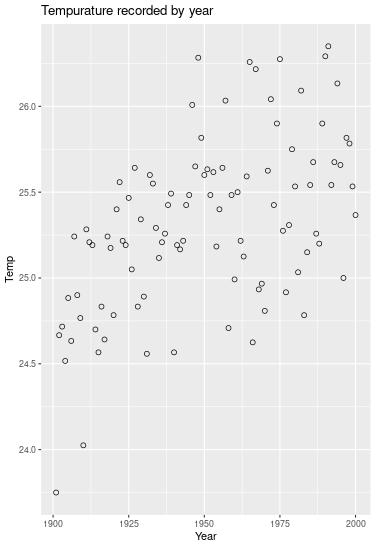
\includegraphics[width=\textwidth]{TempByYear.png}
         \caption{a plot of the KWAMT data}
        \label{fig:KWAMT plot}
    \end{subfigure}
    \hfill
      \begin{subfigure}[b]{0.4\textwidth}
          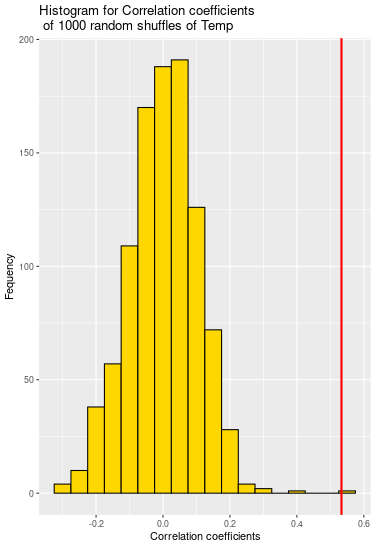
\includegraphics[width=\textwidth]{CorrelationFrequency.png}
         \caption{Histogram showing distribution of Correlation Coefficients}
        \label{fig:Coefficient histogram}
    \end{subfigure}
  
   
    
\end{figure}

\section{Conclusion}
From our results we can see our original data is significantly different from random (p=0) telling us that Florida is getting hotter.

\end{document}